%%%%%%%%%%%%%%%%%%%%%%%%%%%%%%%%%%%%%%%%%%%%%%%%%%%%
%%%% En-tête leçon
\begin{headerBlock}
  \chapter{Phénomènes interfaciaux impliquant des fluides}
    \label{LP_PhenomenesInterfaciaux}
\end{headerBlock}

%%%%%%%%%%%%%%%%%%%%%%%%%%%%%%%%%%%%%%%%%%%%%%%%%%%%
%%%% Références
\begin{center}
\begin{tabularx}{\textwidth}{| X | X | c | c |}
  \hline
  \rowcolor{gray!20}\multicolumn{4}{c}{Bibliographie de la leçon : } \\
  \hline 
  Titre & Auteurs & Editeur (année) & ISBN \\
  \hline
 Gouttes, bulles, perles et ondes & David Quéré, Françoise Brochard-Wyart et Pierre-Gilles de Gennes & \'Editions Belin (2002) &    \\
  \hline 
 Hydrodynamique physique & \'Etienne Guyon, Jean-Pierre Hulin et Luc Petit  &  CNRS ÉDITIONS (3ème édition) &    \\
  \hline 
Notes de cours sur les fluides (2019-2020) & Marc Rabaud  &  Site agreg Montrouge  &    \\
  \hline 
 Why is surface tension a force parallel to the interface? \url{https://arxiv.org/abs/1211.3854} & Marchand, A., Weijs, J. H., Snoeijer, J. H., \& Andreotti, B   & American Journal of Physics (2011)  &    \\
  \hline
  Ce que disent les fluides & Guyon, Hulin, Petit & & \\
  \hline
  Toute la physique dans un verre d'eau & Clément Santamaria & Ellipses (2005) & \\
  \hline
  Thermodynamique & B. Diu & Hermann (2007) & \\
  \hline 
\end{tabularx}
\end{center}

\begin{reportBlock}{Commentaires des années précédentes :}
    \begin{itemize}
        \item \textbf{2014 :} Le lien avec les potentiels thermodynamiques n’est pas souvent maîtrisé. Il est important de dégager clairement l’origine microscopique de la tension superficielle. Le jury constate que trop souvent les candidats présentent des schémas où la représentation des interactions remet en cause la stabilité mécanique de l’interface. Le jury apprécie les exposés dans lesquels le/la candidat(e) ne se limite pas à la statique.
    \end{itemize}
\end{reportBlock}
%%%%%%%%%%%%%%%%%%%%%%%%%%%%%%%%%%%%%%%%%%%%%%%%%%%%

%%%%%%%%%%%%%%%%%%%%%%%%%%%%%%%%%%%%%%%%%%%%%%%%%%%%
%%%% Plan
\begin{reportBlock}{Plan détaillé}

  \textbf{Niveau choisi pour la leçon :} Licence 3
  \newline
  \textbf{Prérequis} : \begin{itemize}
      \item Forces, travail, énergie
      \item Principe de travaux virtuels
      \item Equation de l'hydrostatique
      \item interactions intermoléculaires
  \end{itemize}
  
  \section*{Introduction}
L'étude des phénomènes interfaciaux permet de répondre à un certain nombre de questions comme : pourquoi est-ce que certains insectes marchent sur l'eau, pourquoi les gouttes et les bulles ont la formes qu'elles ont, pourquoi en TP de chimie, lorsqu'on met un liquide dans un tube, on voit la formation d'un ménisque, pourquoi encore voit-on des flaques et pas des bulles d'eau posée sur le sol ? Ces différentes observations nous amènent en réalité à étudier les propriétés des interfaces liquide/gaz, liquide/solide, solide/gaz ou parfois les 3 en même temps ! Nous allons dans cette leçon essayer d'interpréter ces phénomènes qui nous paraissent somme toute très naturels.

  \section{Tension superficiellle}
  \subsection{Origine microscopique}
  Une molécule en volume subit des interactions attractives de la part de ses voisines qui la stabilisent. Une molécule à l'interface a moins de voisines qu'en-dessous : cette configuration augmente son énergie de la différence $\Delta E = p_{sup}E_{intermolec}-p_{sub}E_{intermolec}$ avec $p$ le nombre de premiers voisins. Attention, ici $E_{intermolec}$ est négatif. Par exemple en configuration carré, $p_{sub}=8$ et $p_{sup}=5$. \textbf{Le fluide ajuste donc sa forme pour exposer le minimum de surface afin de minimiser son énergie. Surface = lieu des contraintes}
  
  \subsection{Définition}
  L'énergie pour nécessaire pour accroître la surface d'une interface d'une quantité $dS$ est égale à ce coût en énergie multiplié par le nombre de molécules en surface qui est lui-même proportionnel à $dS$ :
  \begin{equation}
      \delta W = \gamma dS
  \end{equation}
  avec $\gamma$ le coefficient de tension de surface (J.m$^{-2}$). L'ordre de grandeur de $\gamma$ doit être celui des énergies de liaison divisé par la surface d'interaction de la molécule (typiquement une sphère de rayon quelques $\angstrom$. Ex : pour l'interface eau-air, $\gamma = 72.8$~mJ/m$^2$ à $20^{\circ}$C. \\
  
  \textcolor{green}{slide tableau des valeurs de $\gamma$. On commente le fait que pour les métaux, les énergies de liaison sont plus fortes et donc $\gamma$ est plus grand.}\\

  \textcolor{blue}{Expérience qualitative films de savon sur des surfaces (cubes) : il faut que le système minimise son énergie de surface.}

   Voir Diu Complément 5a. pour l'approche énergétique de la bulle de savon. vidéo bulle d'eau dans l'espace : \url{https://www.youtube.com/watch?v=bKk_7NIKY3Y}. 
   
  \subsection{Force capillaire}

  \textcolor{blue}{Expérience qualitative films de savon sur des surfaces (surface avec ficelle) : si on perce un film de savon, la ficelle se déplace.}
  Le coefficient de tension de surface peut également être vu comme une force par unité de longueur. Pour un film de savon rectangulaire, il y a deux interfaces air-liquide dont les vecteurs normaux à la surface sont opposés. Tout segment $d\mathbf{l}$ dans le plan de cette surface est soumise à deux forces égales et opposées si cette surface est à l'équilibre  :
  \begin{equation}
      d\mathbf{f} = \gamma((\mathbf{+\hat{n}})\wedge d\mathbf{l}) +\gamma((\mathbf{-\hat{n}})\wedge d\mathbf{l})
  \end{equation}
  Cette force est tangeante à la surface et normale au contour séparant les deux systèmes.\\
  
  \textcolor{green}{Vidéo force capillaire }\url{https://www.youtube.com/watch?v=g4c_tj1CccE}.
  
  Permet de répondre à pourquoi le geris peut marcher sur l'eau: les pattes hydrophobes du gerris déforment la surface de l'eau (cf clément Santamaria p60) qui va chercher à retrouver sa forme en appliquant une force capillaire sur les pattes. Comme l'insecte est suffisamment léger, la force arrive à compenser le poids. \\

  \textcolor{red}{Transition : On a vu l'exemple des surfaces planes, on va s'intéresser à présent aux interfaces courbes et on va se poser la question : la pression dans une petite bulle est-elle plus grande ou plus petite que dans une grande bulle ,}
  
 \section{Pression et tension de surface}
 
 \subsection{Loi de Laplace}
 Nous avons ici un générateur de bulle. On va faire une expérience simple en créant deux bulles de tailles différentes. \textcolor{blue}{La petite bulle est "mangée" par la grosse.}
 \begin{center}
     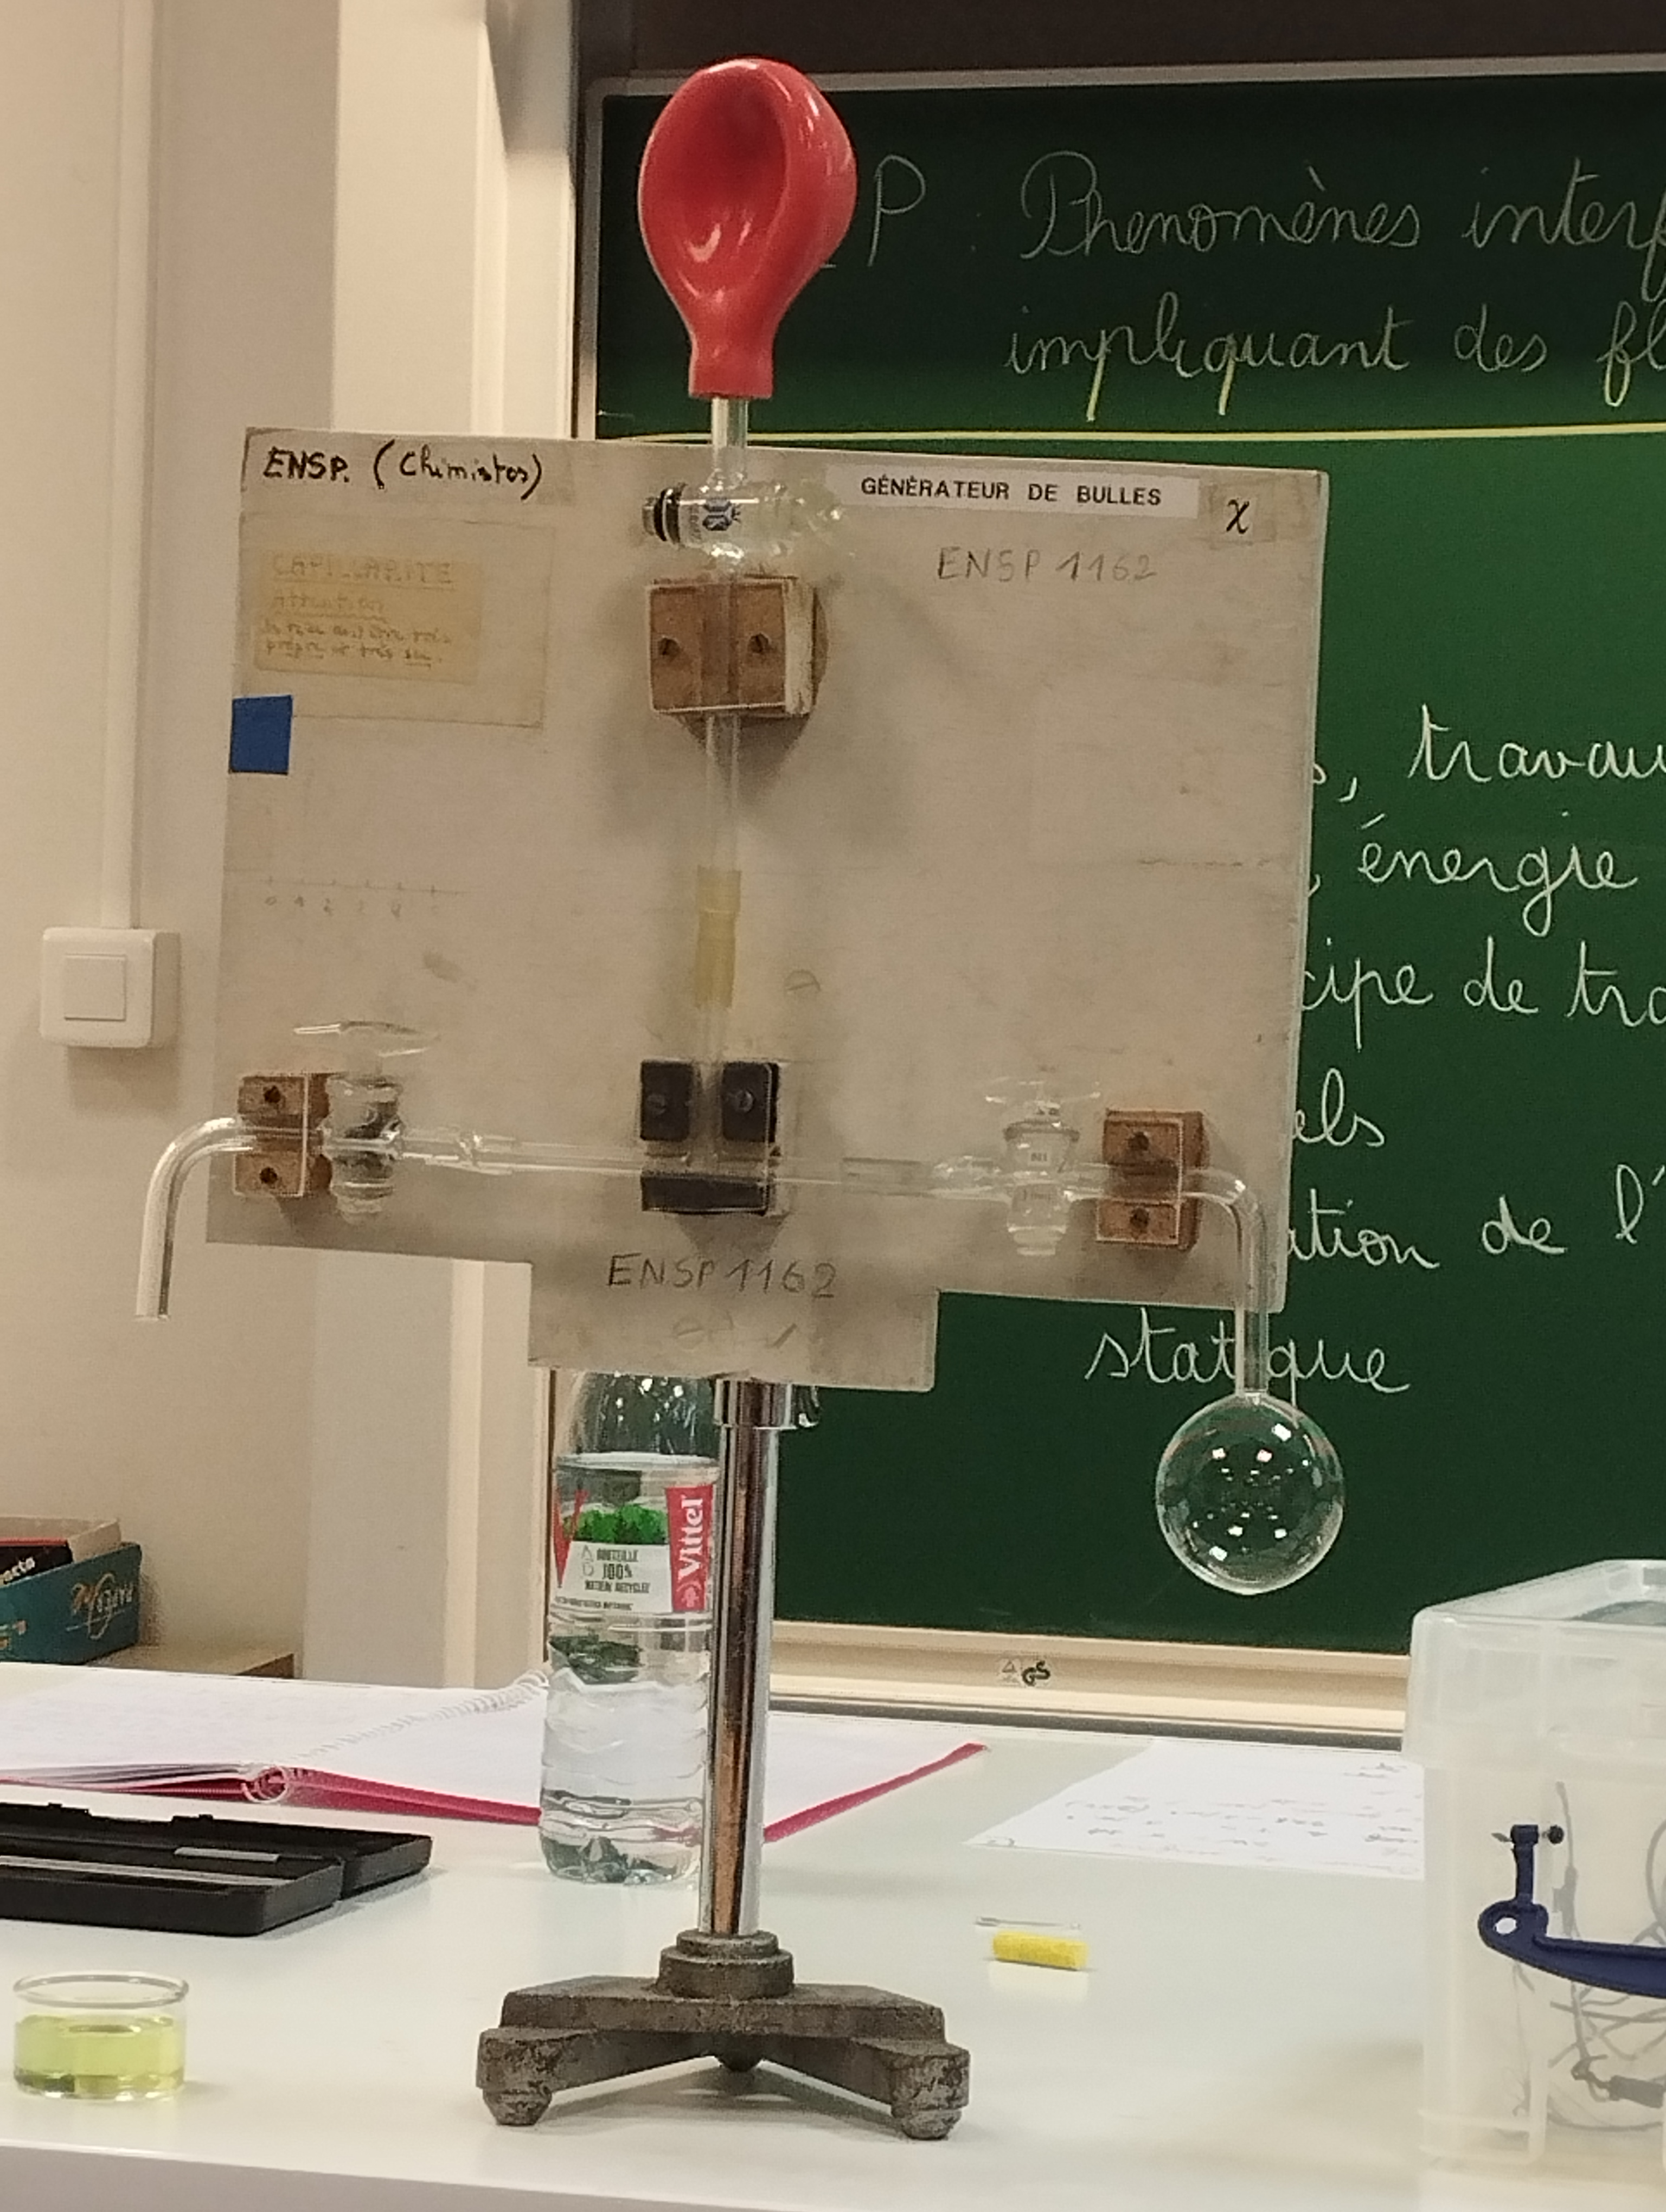
\includegraphics[scale=0.1]{LP_TensionSurface/Manip_Laplace.jpg}
     
 \end{center}
 La différence de pression avec l'extérieur est donc plus grande dans les petites bulles : on peut le démontrer mathématiquement via la \textbf{Loi de Laplace.}
 Pour cela, on applique le principe des travaux virtuels. On imagine qu'on accroît le rayon de la bulle de $dR$ sous une différence de pression $\Delta P = P_1-P_2$ constante. La valeur de $\Delta P$ correspondant à l'équilibre mécanique sera telle que la variation d'énergie totale $\delta W_{tot}$ correspondante est nulle. Celle-ci est la somme du :
 \begin{enumerate}
     \item travail des forces de pression $\delta W_p = -(P_1-P_2)d(\frac{4}{3}\pi R^3)$
     \item la variation d'énergie de surface de la sphère : $\delta W_s = 2d(4\pi R^2\gamma)$, le facteur 2 correspond au fait qu'il y a deux interfaces pour une bulle.
 \end{enumerate}
 A l'équilibre : $\delta W_p+\delta W_s =0$.  Finalement : 
 \textcolor{red}{Loi de Laplace : }
 \begin{equation}
     (P_1-P_2)=\frac{4\gamma}{R}
 \end{equation}
 \begin{itemize}
     \item Plus $R$ est petit, plus la pression à l'intérieur est grande. 
     \item Lorsque $R \rightarrow \infty$ (surface plane), on a continuité de la pression.
     \item Cette loi nous permet de mesurer $\gamma$ expérimentalement.
     \item Remarque : pour une goutte, il y a 1 interface liquide-air donc $(P_1-P_2)=\frac{2\gamma}{R})$
 \end{itemize}
 
 \subsection{Mesure de $\gamma_{savon-air}$}
 \textcolor{blue}{Expérience :}  Pour une bulle de savon, deux interfaces donc $\Delta P =\frac{4\gamma}{R}$. On génère une bulle, on mesure son rayon à l'aide d'un pied à coulisse et la pression à l'intérieur grâce à un manomètre différentiel. Il permet de mesurer la différence de pression entre l'intérieur de la bulle et l'extérieur à travers une mesure de tension (piézo). J'ai pris plusieurs points en préparation, je vais en prendre un devant vous. Une regression linéaire $\delta P = \frac{A}{R}$ permet d'obtenir $\gamma$. \textcolor{red}{Tracer plutôt $R=f(\Delta P)$ car incertitude max sur R.}\\

La pente de $\Delta P = 4 \gamma\times 1/R$ donne $\gamma=28.8 \pm 2.2$~mN/m$^2$ qui est plus faible que celle de l'eau dû à la présence d'un tensioactif (savon = tensioactif). Par ailleurs, on retrouve le bon ordre de grandeur pour une eau savonneuse (internet donne $25$~mN/m$^2$). \\

\subsection{Cas général (cette partie peut sauter)}
Faire la démo. 
\begin{center}
    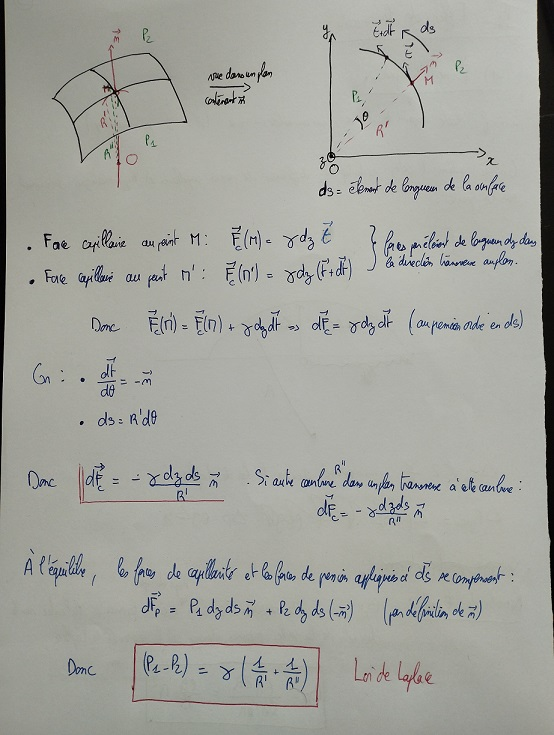
\includegraphics[scale=0.5]{LP_TensionSurface/Demo_Laplace.jpg}
\end{center}
Insister sur le caractère algébrique de R' et R". \textcolor{green}{Slide : Film de savon entre deux anneaux.}
Faire un schéma bulle normale, bulle caténoïde Pour la caténoïde, $\frac{1}{R}=-\frac{1}{R'}$ ce qui permet de satisfaire la loi de Laplace en tout point de l'interface dans le cas ou les pressions sont égales de part et d'autre.\\

\textcolor{red}{Transition : ce qu'on a vu dans cette partie c'est que les effets de capillarité sont directement reliés à la courbure des interfaces pour des petits objets. Mais pour des gros objets, il y a des effets de gravité qui s'ajoutent ce qu'on a vu dans l'expérience avec les bulles de savon.}

  \section{Influence de la gravité}
  
  \textcolor{green}{slide : gouttes de mercure sur une plaque de verre. Plus la taille de la bulle est grande, plus la forme sphérique est déformée.}
  Il y a un effet de gravité qui n'est plus négligeable à partir d'une certaine taille : laquelle ? C'est ce qu'on va voir dans cette partie.
  
  \subsection{Nombre de Bond}
  Considérons une goutte sphérique posée sur une surface plane solide. Cette goutte est plongée dans un fluide de masse volumique $\rho$ et possède une masse volumique $\rho+\Delta\rho$.\\
  
  La différence de pression hydrostatique au point M(z=h) de la goutte est donnée par la loi de l'hydrostatique :
  \begin{align}
      P_1+(\rho+\Delta\rho)gh &= P_2+\rho gh \\
      P_1-P_2 &= \Delta\rho gh = \Delta P_{grav}
  \end{align}
  La différence de pression capillaire à l'interface est donnée par la loi de Laplace :
  \begin{equation}
      P_1-P_2 = 2\frac{\gamma_{LG}}{R} = \Delta P_{cap}
  \end{equation}
  On définit le nombre de Bond $B_O$ comme le rapport entre ces deux différences de pression :
  \begin{equation}
     B_O = \frac{\Delta P_{grav}}{\Delta P_{cap}}\sim \frac{\Delta\rho gr_g^2}{\gamma} = \left(\frac{r_g}{l_c}\right)^2
  \end{equation}
  avec $r_g$ le rayon de la ligne de contact. On a définit ici une longueur appelée longueur capillaire $l_c=\sqrt{\frac{\gamma_{LG}}{\Delta\rho g}}$.
  Cela nous amène à distinguer deux cas :
  \begin{itemize}
      \item Si $l_c>>R$, alors les effets gravitaires sont dominants,
      \item Si $B_O<<1$, l
  \end{itemize}
  Compétition entre gravité et tension de surface : $B_0=\frac{\rho R^2g}{\gamma}$. La longueur capillaire $l_c$ est telle que: $B_0=\frac{\rho l_c^2g}{\gamma}=1$ (frontière entre les deux régimes), soit $l_c = \sqrt{\frac{\gamma}{\rho g}}$.
  Pour l'eau, $l_c=3$mm.\\
  Deux régimes : 
  \begin{itemize}
      \item $R>>l_c$, la gravité domine : goutte plate.
      \item $R<<l_c$, la tension de surface domine, la bulle est sphérique.
  \end{itemize}
  Photo ménisque : résulte de cette compétition entre tension de surface responsable de sa formation et gravité qui s'y oppose. Menisque concave pour un fluide mouillant (ex: eau dans tube en verre) et convexe pour un fluide peu mouillant (ex: mercure dans tube en verre)
  \begin{center}
      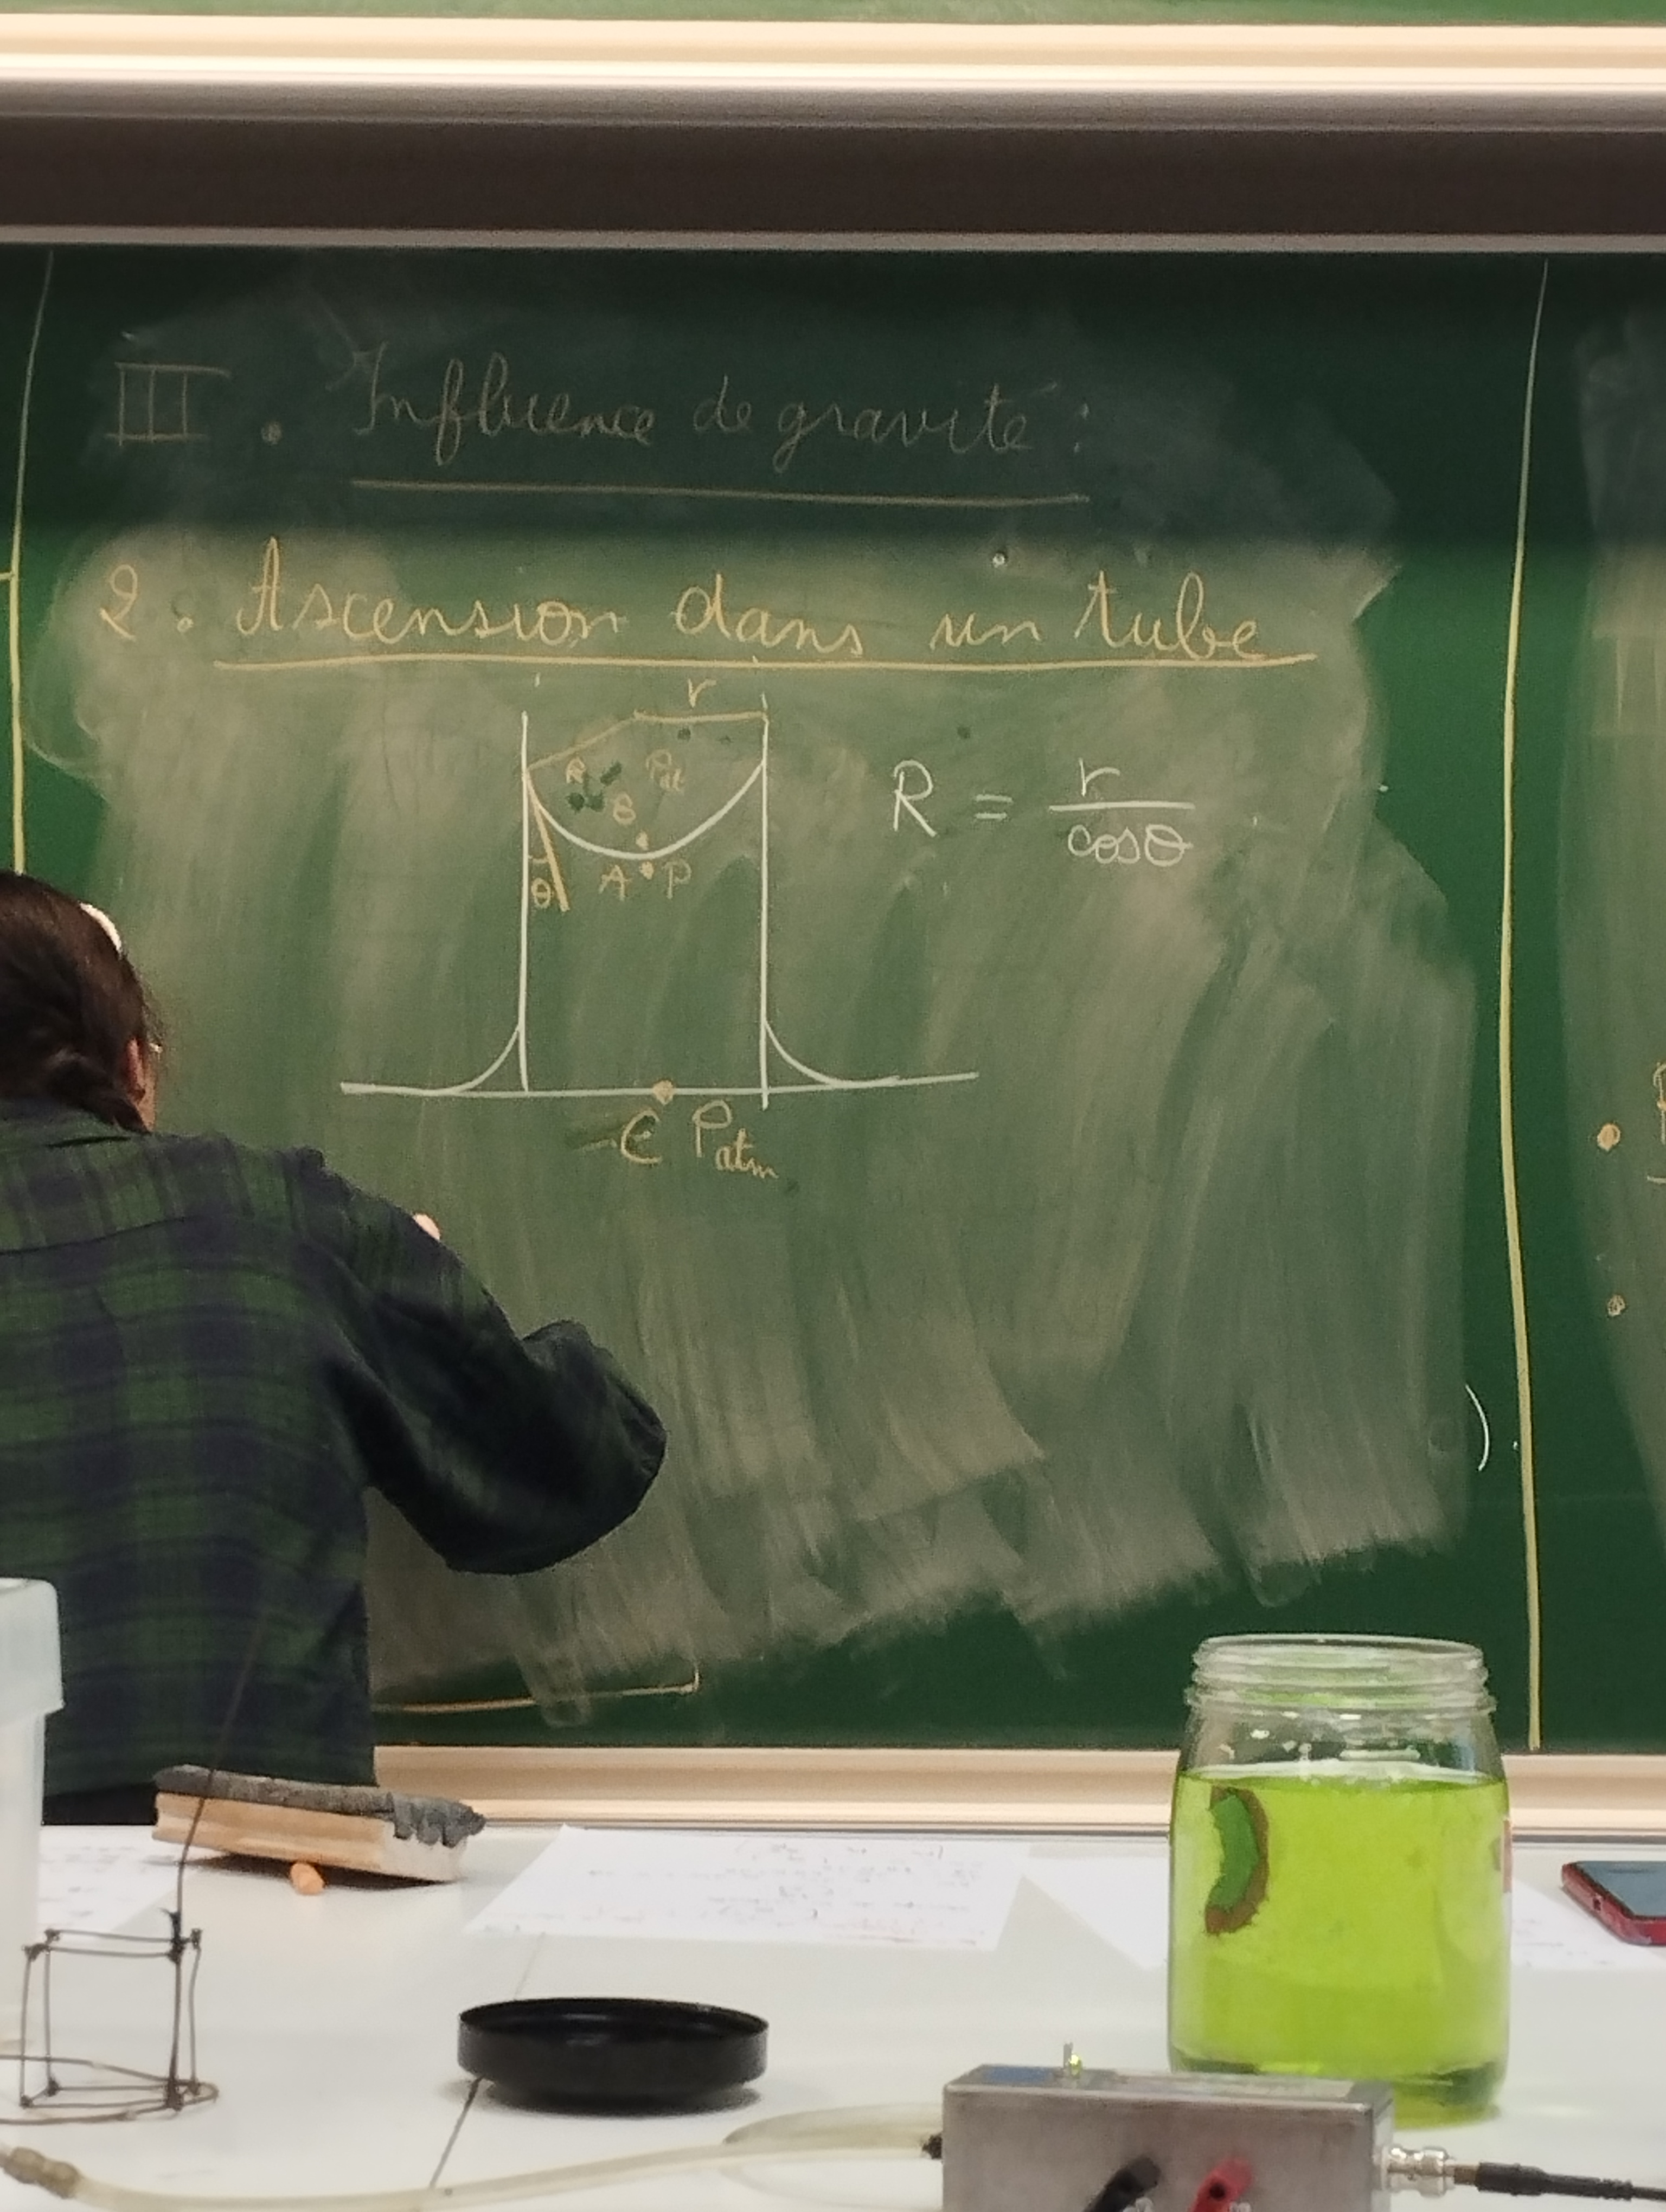
\includegraphics[scale=0.1]{LP_TensionSurface/Menisque.jpg}
  \end{center}

  \subsection{Ascension capillaire dans un tube}
  Vidéo de l'ascension d'un liquide dans différents tubes capillaires (voir site Laurent Le Guillou dans la partie TP). Plus le tube est fin, plus le liquide monte haute.
  Schéma liquide dans un tube de rayon $r$, rayon de courbure du ménisque $R$, angle de contact $\theta$. On applique la loi de Laplace : $\Delta P = \frac{2\gamma}{R}=\frac{2\gamma\cos(\theta)}{r}$. En appliquant l'équation de l'hydrostatique, on obtient \textcolor{red}{la Loi de Jurin} :
  \begin{equation}
      h = \frac{2\gamma\cos(\theta)}{\rho g r}
  \end{equation}
  En effet, plus $r$ est petit, plus $h$ est grand. Cette loi permet de mesurer $\gamma$.

\section{Effet de mouillage}
  \textcolor{green}{Mouillage :} étude de l'étalement d'un liquide sur un substrat (solide ou liquide). Utile dans l'industrie (peinture, encre, traitement des pneus, crème, maquillage, etc.).\\
  $\theta =$ angle de contact, permet de savoir si un liquide mouille plus ou moins bien un substrat. Résulte d'une compétition entre les tensions de surface intervenant dans les trois interfaces (L/G, L/S, S/G). \\
  \textbf{26min}\\
  Le système est \{\textbf{dl}$\in$ ligne triple\}. 
  $\textbf{dF}=0$ à l'équilibre. La projection sur l'axe du solide donne la \textcolor{red}{Loi de Young-Dupré} :
  \begin{equation}
      \gamma_{LG}\cos(\theta) = \gamma_{SG}-\gamma_{SL}
  \end{equation}
  
  \section*{Conclusion (40min)}
  Expérience de conclusion : Pince à nourrice dans eau flotte, puis coule avec tensio-actif (savon).



\end{reportBlock}


%%%%%%%%%%%%%%%%%%%%%%%%%%%%%%%%%%%%%%%%%%%%%%%%%%%%
%%%% Questions
\begin{reportBlock}{Questions posées par l’enseignant (avec réponses)}
  \textbf{C : C'est quoi un tensioactif ?} \textcolor{purple}{\'{E}lément qui diminue la tension de surface. Il est composé d'une tête hydrophile et d'une queue hydrophobe. La tête va se mettre à l'interface du côté de l'eau tandis que la queue sera du côté de l'air, faisant le lien entre l'eau et l'air. Cette configuration permet de diminuer l'énergie de l'interface, et donc diminue la tension de surface. } \newline

  \textbf{C : La dynamique de l'ascension dans la loi de Jurin semble diférrente en fonction du diamètre du tube ? Pouvez-vous discuter des éléments à prendre en compte pour essayer de comprendre pourquoi ça monte plus vite ou plus lentement ?} \textcolor{purple}{Plus le rayon est grand, plus la vitesse est grande. Peut se comprendre en ordre de grandeur via $\nabla P = \eta \Delta v$ soir $\frac{P}{h} \sim \eta \frac{v}{r^2}$}
  %En comparant à Poiseuille cylindrique, il y a une dépression à l'interface air/liquide qui fait augmenter brutalement la vitesse. Lorsque le liquide monte, le gradient de pression diminue ($\frac{\delta P}{\delta z}=\frac{2\gamma}{rh}$, r rayon du tube et h hauteur de l'ascension) et en prenant en compte la gravité et les forces de viscosité ($\frac{\delta^2v_r}{\delta z^2}$), ça va ralentir l'ascension.

  \textbf{C : Où placeriez-vous cette leçon dans le cours global de mécanique des fluides ?} \textcolor{purple}{Après l'équation de Navier-Stokes. C'est presque une domaine un peu à part.}

  \textbf{C : Peut-on imaginer qu'on n'ait pas de saut de pression à travers une surface courbe ?} \textcolor{purple}{En utilisant l'équation de Laplace pour une surface quelconque, $\Delta P =\gamma(1/R+1/R')$, R et R' sont les deux rayons de courbures de la surface en un point donné et sont algébriques (compté positivement si le centre de la coubure est à l'intérieur de la surface, négativement sinon. Par exemple, pour un point selle, on a $R' = -R$ impliquant une continuité de la pression.}

  \textbf{C : Dans l'équation de Young-Dupré, vous avez dessiné 3 forces mais il ne me semblait pas qu'on était en équilibre (au moins à la normale à la surface)} \textcolor{purple}{La force de réaction du support compense la composante normale de la force de tension de surface.}

  
  \textbf{C : D'autres façon pour déterminer $\gamma$ ?} \textcolor{purple}{Tensiomètre à plaque de Wilhelmy: on mesure la force exercée sur la plaque par le liquide grâce à une microbalance, et on peut en déduire $\gamma$.}

  
  \textbf{C : Dessin d'une goutte sur un plan incliné ? De quoi dépendrait l'angle d'inclinaison ?} \textcolor{purple}{Vitesse, viscosité, et coefficient de tension de surface.}

  
  \textbf{C : Pouvez-vous expliquer pourquoi on peut faire des chateaux de sables avec du sable mouillé ?} \textcolor{purple}{La présence d'eau va créer un pont capillaire entre deux grains qui va augmenter la force de cohésion entre les grains. Cette cohésion se fait sur une surface beaucoup plus grande pour le grain mouillée grâce au pont capillaire alors que pour un grain sec, cette cohésion se fait au niveau d'une rugosité (très petite surface) et donc insuffisance pour maintenir un château de sable.}



  \textbf{C : Pourquoi les serviettes sont rêches quand elle sèche ? Quel est le principe d"un adoucissant ?} \textcolor{purple}{Lorsqu'une serviette est mouillée, l'eau va chercher à minimiser son interface avec l'air en collant et écrasant les fibres de la serviette (c'est aussi pour ça que nos cheveux sont collés en sortant de la douche). En séchant, la serviette durcit, lui donnant une texture rêche. L'adoucissant agit chimiquement sur les fibres pour rendre le linge plus doux au toucher.}


  \textbf{C : $\gamma(T)$ ? Que se passe-t-il s'il y a des endroits du fluide qui sont plus chauds que d'autres ?} \textcolor{purple}{Création d'un gradient de tension de surface qui va causer un déplacement du liquide des zones de faibles $\gamma$ vers les zones de $\gamma$ élevée (cf. effet Marangoni).}

  
  \textbf{C : On parle parfois de liquide mouillant et de liquide non-mouillant. Valeurs de $\theta$ ?} \textcolor{purple}{Mouillage total : $\theta=0$, non-mouillage total : $\theta=\pi$.}

  
  \textbf{C : Commenter les incertitudes sur l'expérience ?} \textcolor{purple}{Incertitudes dominantes sur la mesure du rayon avec le pied à coulisse que j'ai pris de $0.5$mm, ce qui est une grande incertitude.}


  \textbf{C : Principe du manomètre ?} \textcolor{purple}{Un piézoélectrique subit une contrainte mécanique sous l'effet de la différence de pression, générant une tension que l'on mesure. Le constructeur nous donne la relation de conversion entre tension et pression.}

  \end{reportBlock}
  
%%%%%%%%%%%%%%%%%%%%%%%%%%%%%%%%%%%%%%%%%%%%%%%%%%%%
%%%% Commentaires
\begin{reportBlock}{Commentaires lors de la correction de la leçon}
Bonne leçon, beaucoup apprécié toutes les expériences montrées. Vous maîtrisez pas mal de choses. Attention à ce que le dispositif ne gène pas la vue sur le tableau.\\


\end{reportBlock}



%%%%%%%%%%%%%%%%%%%%%%%%%%%%%%%%%%%%%%%%%%%%%%%%%%%%
%%%% Correction
\begin{reportBlock}{Partie réservée au correcteur}
  \textbf{Avis général sur la leçon (plan, contenu, etc.) :}
  
  
  \textbf{Notions fondamentales à aborder, secondaires, délicates :}
  
  
  \textbf{Expériences possibles (en particulier pour l'agrégation docteur) :}
  
  
  \textbf{Bibliographie conseillée :}
\end{reportBlock}


\begin{reportBlock}{Partie réservée au correcteur}
  \textbf{Avis général sur la leçon (plan, contenu, etc.) :}
  
  
  \textbf{Notions fondamentales à aborder, secondaires, délicates :}
  
  
  \textbf{Expériences possibles (en particulier pour l'agrégation docteur) :}
  
  
  \textbf{Bibliographie conseillée :}
\end{reportBlock}